\documentclass[12pt]{article}

\usepackage{microtype}
\usepackage{todonotes}
\usepackage{siunitx}
\usepackage{graphicx}
\usepackage{tikz}
\usepackage{pgfplots}
\usepackage[section]{placeins}
\usepackage[marginparwidth=1.75in,left=0.5in,right=2in]{geometry}
\usepackage{hyperref}

\usetikzlibrary{patterns}
\graphicspath{ {./figs/} }
\pgfplotsset{compat=1.13}
\makeglossaries



\title{Master's Thesis}
\author{
        Nathan Pemberton \\
                Department of Computer Science \\
                University of California at Berkeley
}
\date{\today}

\begin{document}
\maketitle

\newpage

\begin{abstract}

Researchers from industry and academia have recently proposed to disaggregate
memory in warehouse-scale computers, motivated by the increasing performance of
networks, and a proliferation of novel memory technologies. In a system with
memory disaggregation, each compute node contains a modest amount of fast
memory (e.g.  high-bandwidth DRAM integrated on-package), while large capacity
memory or NVM is made available across the network through dedicated memory
nodes. One common proposal to harness the fast local memory is to use it as a
large cache for the remote bulk memory. This cache could be implemented purely
in hardware, which could minimize latency, but may involve complicated
architectural changes and would lack OS insights into memory usage.  An
alternative is to manage the cache purely in software with traditional paging
mechanisms. This approach requires no additional hardware, can use
sophisticated algorithms, and has insight into memory usage patterns. However,
our experiments show that even when paging to local memory, applications can be
slowed significantly due to the overhead of handling page faults, which can
take several microseconds and pollute the caches. In this thesis, I propose a
hybrid HW/SW cache using a new hardware device called the ``page fault
accelerator'' (PFA), with a special focus on the impact on operating system
design and performance. With the PFA, applications spend 2.5x less time
managing paging, and run 40\% faster end-to-end.
\end{abstract}



\newpage
\tableofcontents
\newpage

\section{Introduction} \label{sec_intro}
    Traditional data center design aggregates all necessary resources (e.g., disk,
memory, power supply, etc.) into many self contained server chassis. This
design was motivated by the ability to leverage commodity PC components and
networks\cite{NOW}.  Additionally, an aggregated design was desirable because
in-chassis interconnects were significantly faster than networks. However,
data center-side compute has grown into an important independent market, leading
to specialized server platforms and networks (often called \glspl{wsc}).
Furthermore, networking technology has seen a rapid increase in performance,
with \SI{40}{\giga\bit\per\second} Ethernet becoming commonplace, and 100+ \si{\giga\bit\per\second} networks readily
available, narrowing the gap between off-package DRAM and remote
memory\todo{what is this paper called? why does my zotero not have it?}.
Workloads have also changed; applications are fundamentally distributed (e.g.,
service-oriented architecture, map-reduce, etc.), use larger and rapidly
changing datasets (``Big Data''), and demand latencies that can only be
delivered by in-memory processing. Finally, a number of promising new memory
technologies are becoming available. New \gls{nvm} devices are being
introduced that promise low idle power, high density, and near-DRAM performance
(e.g., fast NAND, phase-change, memristor). On the high-performance side,
improvements in packaging technology have led to fast on-package DRAM (e.g.,
HBM) that offers hundreds of GB/s of bandwidth with capacities in the tens of
GB.

These hardware and software trends have lead to proposals from both
academia\cite{firebox}\cite{dredbox} and
industry\cite{themachine}\cite{huaweidc30}\cite{intelrsa}\cite{fbdisag} for a
new style of \gls{wsc} where resources are disaggregated \glsadd{disag}.  In a
disaggregated \gls{wsc}, resources like disk and memory become first-class
citizens over a high-performance network. A compute node couples CPUs, network
interfaces, and a small amount of high-speed memory into a self-contained
\gls{sip}. This design allows data center operators to scale memory capacity,
while allocating it more flexibly (avoiding stranded resources and complex
resource allocation policies). However, the memory access latency will be
higher than traditional off-package DRAM, and bandwidth may be limited or
subjected to congestion. The small on-package memory allows us to mitigate some
of this performance gap, but the question remains: how best to use it?

One way to harness the on-package DRAM is to use it as a large cache for remote
bulk memory. Operating systems have traditionally provided this through virtual
memory \gls{paging} which uses virtual memory to treat local physical memory as
a software-managed cache (typically for disk). Indeed, several recent academic
research projects have proposed using paging over \gls{rdma} as a way of
disaggregating memory\cite{infiniswap}\cite{osdidisag}. Paging has
traditionally been backed by slow disks with access latencies in the
milliseconds. This lead to sophisticated algorithms that can take several
microseconds for every cache miss. An alternative is to have fully hardware
managed DRAM caches\cite{volos_DRAM}\cite{lee_tagless}. These eliminate much of
the overhead, but lack the sophistication and application-level insight of
OS-based approaches. For example, operating systems often use significant
memory for optimistic pre-fetching and caching of disk blocks. A
hardware-managed cache may choose to store these in remote memory, while the OS
would simply delete them.

This thesis introduces a hardware accelerator for OS-managed caching called the
\gls{pfa}. The \gls{pfa} works by handling latency-critical page faults
(cache-miss) in hardware, while allowing the OS to manage latency-insensitive
(but algorithmically complex) evictions asynchronously. We achieve this
decoupling with a queue of free page frames (freeQ) to be used by the \gls{pfa}
for fetched pages, and a queue of new page descriptors (newQ) that the OS can
use to manage new page meta-data. Execution then proceeds as follows:

\begin{itemize}
	 \item The OS allocates several page frames and pushes their addresses onto
		 the \emph{freeQ}.
   \item The OS experiences memory pressure and selects pages to evict to
		 remote memory. It marks them as ``remote'' in the page tables and then
     provides them to the \gls{pfa} for eviction.
   \item The application attempts to access a remote page, triggering the
     \gls{pfa}
		 to request the page from remote memory and place it in the next
		 available free frame. The application is then resumed.
	 \item Some time later (either through a background daemon, or through an
		 interrupt due to full queues) the OS pops all new page descriptors off
		 the \emph{newQ} and records the (now local) pages in its meta-data. The
		 OS typically provides more free frames at this time.
\end{itemize}




\section{Motivation}
    \subsection{FireBox} \label{sec_firebox}
        While there are several proposals for a disaggregated \acrlong{wsc}, we will use the
Firebox\cite{firebox} project as an example throughout this thesis (see Figure
\ref{fig:fb_diagram}). The Firebox proposal incorporates ideas from several academic and industrial projects and is representative of disaggregated \glspl{wsc} in general.

\begin{figure}
    \centering
    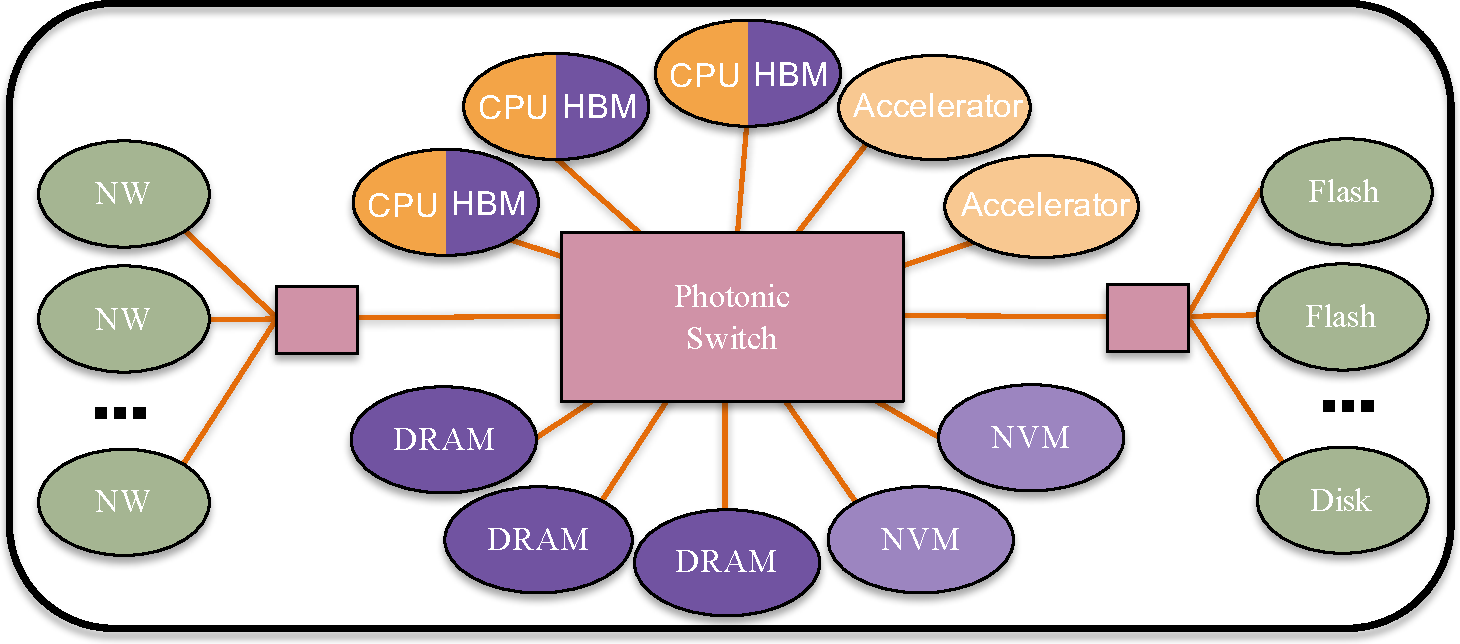
\includegraphics[width=0.9\columnwidth]{figs/FBDiagram.pdf} \label{fig:fb_diagram}
    \vspace{-5mm}
    \caption{The Firebox WSC proposal. Compute and memory resources become first-class citizens over a high-radix network, allowing flexible resource allocation and scaling. Lower-speed peripherals (such as disk or wide-area networking} can be connected farther away in the network topology.
\end{figure}

Firebox proposes using high-bandwidth, high-radix, networks to
connect compute, memory, and storage nodes in a WSC. Firebox does not dictate any particular networking technology, but is motivated by emerging integrated silicon photonic network
interfaces because they can be integrated directly on-die (or on package, e.g., \gls{sip}), minimizing pin-out and
providing high bandwidth at low power. By multiplexing many wavelengths onto a
single fiber (wave-division multiplexing), it is possible to create a very high
fanout while using few physical interfaces. This fanout may enable very high
radix switches that can connect many SiPs within a single hop. Current
estimates indicate these photonic networks can achieve aggregate bandwidths
exceeding \SI{1}{\tera\bit\per\second} over 128 channels on a single
fiber\cite{naturePhotonic}\cite{Photonic09}. Link latencies (including photonic
transceiver crossings) are on the order of 10s of \si{\nano\second}, but final
latencies will be determined by protocol decisions. We believe round-trip
latencies (across a single switch) of approximately \SI{1}{\micro\second} to be
a conservative prediction. For reference, current infiniband EDR networks
provide approximately \SI{24}{\giga\bit\per\second} per link (with up to 12
links per NIC), and have round-trip latencies of approximately
\SI{2}{\micro\second}\cite{binnigNW}.

Compute nodes can be CPUs or special-purpose accelerators. In either case, they
will include some amount of high-bandwidth on-package memory (HBM), we
typically assume densities of approximately \SI{2}{\giga\byte} per core. This
on-package memory will have very high speed (up to
\SI{1}{\tera\byte\per\second}, at much lower power than traditional off-package
memories. A relatively large amount of on-package memory, coupled with very
fast networks allows most memory in the system to consist of network-attached memory
blades which are optimized for cost, power, and density. The total available
memory may be as much as \SI{1}{\peta\byte}. Other resources may also be used,
such as high-performance NAND flash, disks, and external network bridges.
Ultimately, the scale of such a system will be limited by network capacity, but
a Firebox would include at least thousands of cores and hundreds of
\si{\tera\byte} of bulk memory.

\paragraph{WSC Challenges} \Glspl{wsc} promise to lower \gls{tco} significantly
by improving utilization and allowing components to develop and scale
independently. These benefits bring with them opportunities and challenges that
bear mentioning. The increased flexibility in resource allocation will require
sophisticated and scalable resource management algorithms that balance
utilization, congestion, and fairness. Encryption and authentication keys will
also need to be managed to protect memory traffic that is now exposed to
attackers across the network. In addition to being secure, memory-like
interfaces must be very high performance and any encryption or authentication
mechanisms must match that performance.  Finally, this new heterogeneous memory
hierarchy presents challenges to applications and operating systems. What is
the right interface to expose the gap between local and remote memory? Will
applications need to be re-written to take advantage of it? It is these
questions that I focus on in the remainder of this thesis.


    \subsection{Interfaces to Remote Memory} \label{sec_rmemApproaches}
        The problem of deep and heterogeneous memory hierarchies is not entirely new;
previous mainframe and high-performance computing platforms have previously
exposed the concept of remote memory. I will describe some of these approaches
in the next two sections.

\subsubsection{Low-Level Interfaces}
\paragraph{NUMA}
\Gls{numa} architectures partition memory resources across several compute
nodes such that memory is always local to exactly one compute resource, but
still directly addressable by the others. In this case, all memory has the same
interface (loads and stores from CPUs), but some is faster than others
(non-uniform). Some \gls{numa} systems include hardware services to aid in page
migration to mitigate this effect\cite{sgi_origin}.

\Gls{numa} systems are appealing because they appear to software as a single,
large memory. They can also offer memory access latencies on the order of 100s
of nanoseconds. This performance and tight coupling, however, limit
scalability. \Gls{numa} the largest NUMA systems can scale to hundreds of nodes
and 10s of TB of memory\cite{sgiUV}, but typical systems support only a few TB
and less than 10 nodes (due to poor scaling in cost and power).

\paragraph{RDMA}
\gls{rdma} systems are similar to NUMA in that memory resources are partitioned
among several compute nodes (memory is always local to
someone)\cite{RoCE}\cite{RFC5040}. The difference is that while NUMA systems
typically expose a cache-coherent load-store interface to both local and remote
memory resources, \gls{rdma} uses a special put/get interface to access remote
memory resources.  Typically, this service is provided through the network
interface and managed by software. This interface allows RDMA systems to scale
beyond what is possible in NUMA systems, at the cost of remote memory access
performance and a more complex interface to applications.

\Gls{rdma} systems can scale to thousands of nodes and petabytes of
memory\cite{IB_ref_design}. Performance can vary, and scales with deployment
size, but modern Infiniband networks provide round-trip latencies of several
microseconds (within a rack) and bandwidths of hundreds of gigabytes per
second\cite{ib_perf}. These systems have historically been considered costly
and only were primarily deployed in supercomputing environments, but recent
Ethernet-based implementations have made them increasingly
accessible\cite{RoCE}.
 
\paragraph{Memory Semantic Fabrics}
Finally, a new class of interface has been recently introduced; the
memory-semantic fabric. A memory-semantic fabric abstracts memory into a simple
load-store interface (rather than technology-specific protocols). This
abstraction enables heterogenous memory technologies in flexible topologies.
Memory thus becomes a first-class citizen (often called a "memory blade") on a
memory-optimized interconnect. The hope is that such interfaces will allow for
greater scalability and flexibility than NUMA, while providing a more direct
interface than RDMA. There are several commercial consortia developing
cache-coherent interconnects for integrating accelerators and memories within a
rack \cite{ccix}\cite{capi}. Some academic projects have focused on scaling
NUMA by increasing the level of abstraction (e.g.,
\cite{sonuma}\cite{lim_disag}).  Finally, an industrial effort called Gen-Z
provides a more general interface that can connect memory, accelerators, and
storage using memory-oriented operations (like load and store)\cite{genz}.
While Gen-Z does not include cache-coherence in the core specification, it can
be added through custom commands between devices that require it. It remains to
be seen how these new interconnects balance performance, scalability, and cost.

\subsubsection{Software Interfaces} The low level interfaces listed above do
not necessarily mandate a particular software interface. NUMA systems typically
expose a virtual memory abstraction to applications. In this case, the OS
manages mappings from virtual to physical addresses while hardware uses those
mappings to automatically route loads and stores to the appropriate memory
resources. The OS is also responsible for choosing which NUMA domain to
allocate memory from. This can be a complex decision and much effort has gone
into studying such allocation policies\cite{linux_numa}.

RDMA systems are further divorced from specific hardware interfaces and enjoy a
great diversity of interfaces. Some programming languages use a partitioned
global address space to make it appear as if language-level variables are all
directly accessible\cite{upc}\cite{grappa}. Other systems use RDMA more
directly to accelerate applications such as key-value
stores\cite{ramcloud}\cite{farm}.

Memory-semantic fabrics are newer and it is not clear how their interfaces
should be exposed. By coupling tightly with CPUs, it is possible to address
them directly using virtual memory. However, it may be desirable to allow
applications to choose which memory they access, or have more abstracted
interfaces (e.g., disk-like).

In this thesis, I will focus on a very general interface called demand paging
(covered in detail in the next section) that can be implemented under any of
the low-level interfaces listed here. However, the focus will be on the
memory-semantic fabric approach.


        
\section{Page Fault Accelerator} \label{sec_pfa}
    \subsection{OS Paging Overview} \label{sec_pagingOverview}
        Many architectures expose the abstraction of virtual memory. While the
implementation of virtual memory is fairly similar across architectures and
operating systems, for concreteness I will use the RISC-V ISA (privileged
architecture version 1.10\cite{riscv_priv110}), and Linux version
4.15\cite{linux} for most examples in this thesis.

With virtual memory, the addresses issued through load and store instructions
do not directly correspond with physical address on the memory bus. Instead,
they are translated to physical addresses through a data structure called the
\gls{pgtbl} (see Figure \ref{fig:generic_paging}).  Page tables contain
translations for fixed-sized ranges of memory called \glspl{page} (\SI{4}{\kibi\byte}
in RISC-V). In addition to translations, each \gls{pte} contains meta-data about the page such as read/write permissions, page
validity, and whether the page has been read or written to recently (called
``accessed'' and ``dirty'' respectively). Throughout this thesis I will refer to
the logical group of data as a ``page'' and the physical region of memory
containing that page as a ``page frame'' or simply ``frame''.  

\begin{figure}[h]
    \centering
    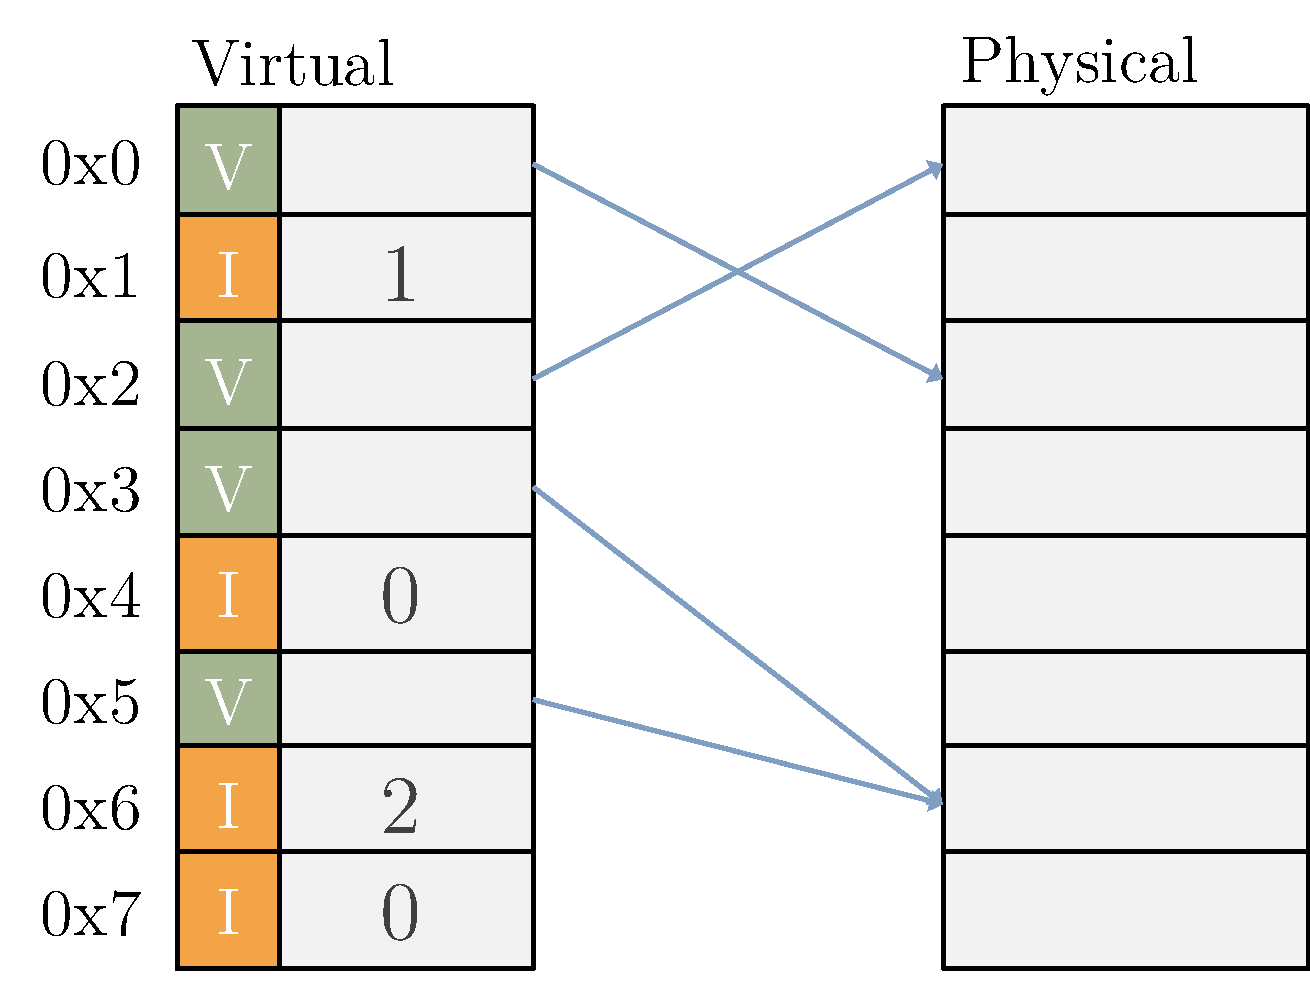
\includegraphics[width=0.5\columnwidth]{figs/generic_page_table.pdf}
    \vspace{-5mm}
    \caption{Example page-table. Entries with a ``V'' are valid (have the valid
             bit set) while ``I'' indicates an invalid entry (valid bit clear).
           Addresses refer to virtual page number (the 52 most significant bits
         in RISC-V).}
    \label{fig:generic_paging}
\end{figure}

Figure \ref{fig:generic_paging_flow} shows a flow chart for translating a page:

\begin{outline}[enumerate]
  \1 The CPU issues a load or store for a particular virtual address
  \1 The load/store unit queries a small cache of recently used translations
  called the \gls{tlb}.
    \2 If the translation is found, a physical address is returned to the CPU
    which then performs the memory access.
  \1 If the translation is not found, the TLB uses a hardware block called the
  \gls{ptw} to find the relevant PTE in main memory.
    \2 If the PTE is marked valid, the physical address is returned to both the
    TLB (for caching) and the CPU.
  \1 If the PTE is marked invalid, the PTW issues a page-fault to the CPU which
  then traps into the OS to handle the invalid memory access.
\end{outline}

\begin{figure}[h]
    \centering
    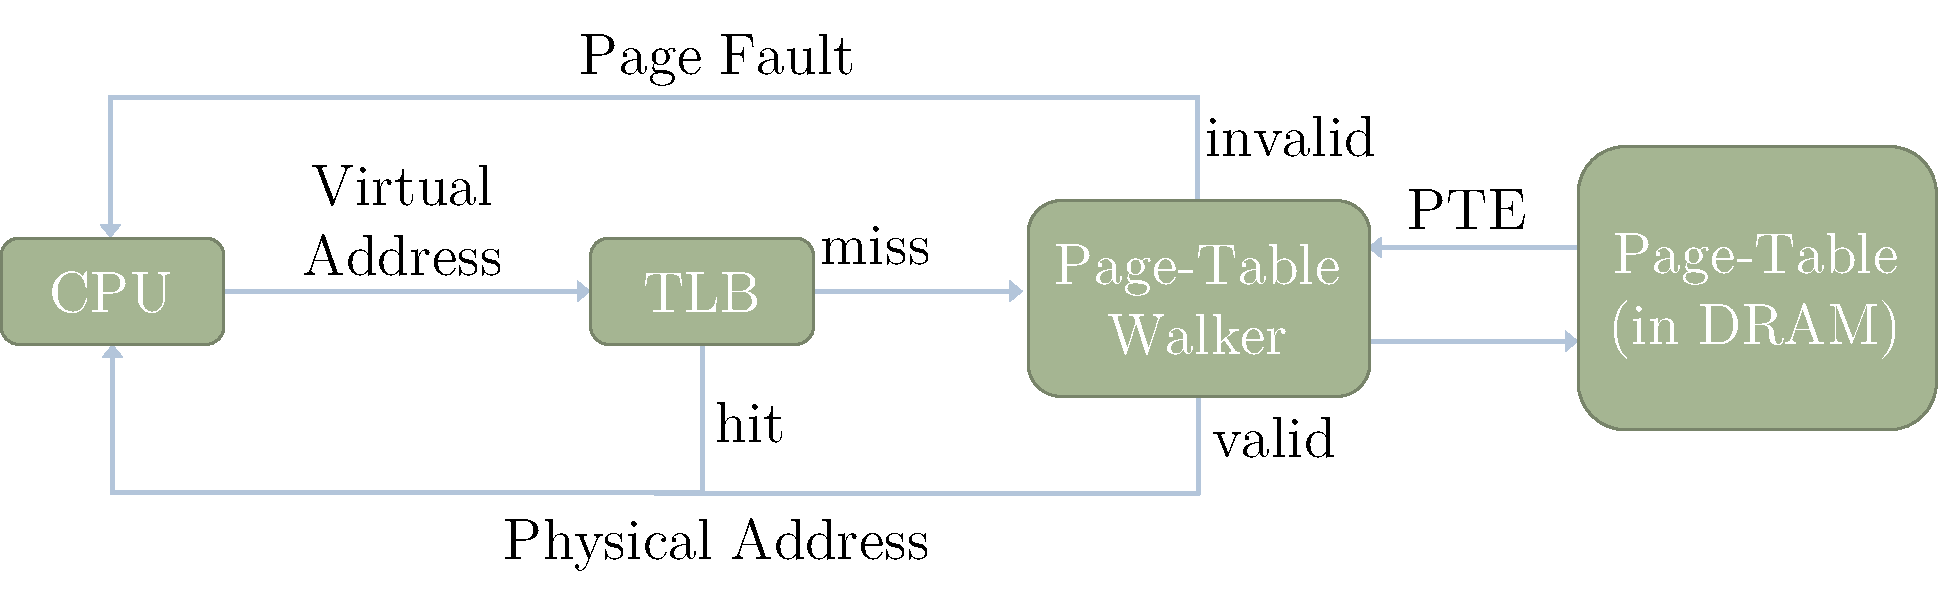
\includegraphics[width=0.9\columnwidth]{figs/generic_paging.pdf}
    \vspace{-5mm}
    \caption{Flow chart for virtual to physical address lookup.}
    \label{fig:generic_paging_flow}
\end{figure}

In addition to providing memory protection and dirty/accessed tracking, virtual
memory enables a number of operating system techniques to manage physical
memory through the page-fault mechanism. For example, new virtual memory
allocations in Linux do not get physical addresses assigned immediately.
Instead, the OS protects all reads and writes to the page, and only allocates
memory if and when the process actually attempts to use it (virtual address 0x4
in Figure \ref{fig:generic_paging} for example). This saves considerable memory
allocation overheads when processes allocate more memory than they actually use
(a fairly common occurrence). Another technique, called paging, creates the
appearance of unlimited memory by transparently moving pages to an external
storage device (such as a hard disk) and bringing them back only when accessed.
This effectively turns main memory into a software-managed cache for the
external storage device. It does this by marking the evicted pages as
``invalid'', and storing their location on the storage device in the PTE. For
example in Figure \ref{fig:generic_paging}, virtual pages 0x1 and 0x6 are
currently stored on an external storage device at index 1 and 2, respectively.

    \subsection{Page Fault Accelerator Design} \label{sec_pfaDesign}
        The primary interface to the PFA is through a number of memory-mapped queues:
\gls{freeq}, \gls{newq}, and \gls{evictq}. The \gls{freeq} contains unused page frames that the PFA can
use for fetching new pages, the \gls{newq} reports any recently fetched pages to the
OS bookkeeping thread, and the \gls{evictq} contains a list of local pages that
should be stored in remote memory. Using these queues, execution proceeds as
follows:

\paragraph{Eviction}
The PFA handles all communication with the memory blade. This includes page
eviction. The basic procedure is as follows (see figure \ref{fig:evict_detail}
for a detailed description):

\begin{outline}[enumerate]
    \1 The OS identifies pages that should be stored remotely.
    \1 It evicts them explicitly by writing to the \gls{evictq}.
    \1 The OS stores a page identifier in the PTE and marks it as remote.
\end{outline}

\begin{figure}[h] \centering
  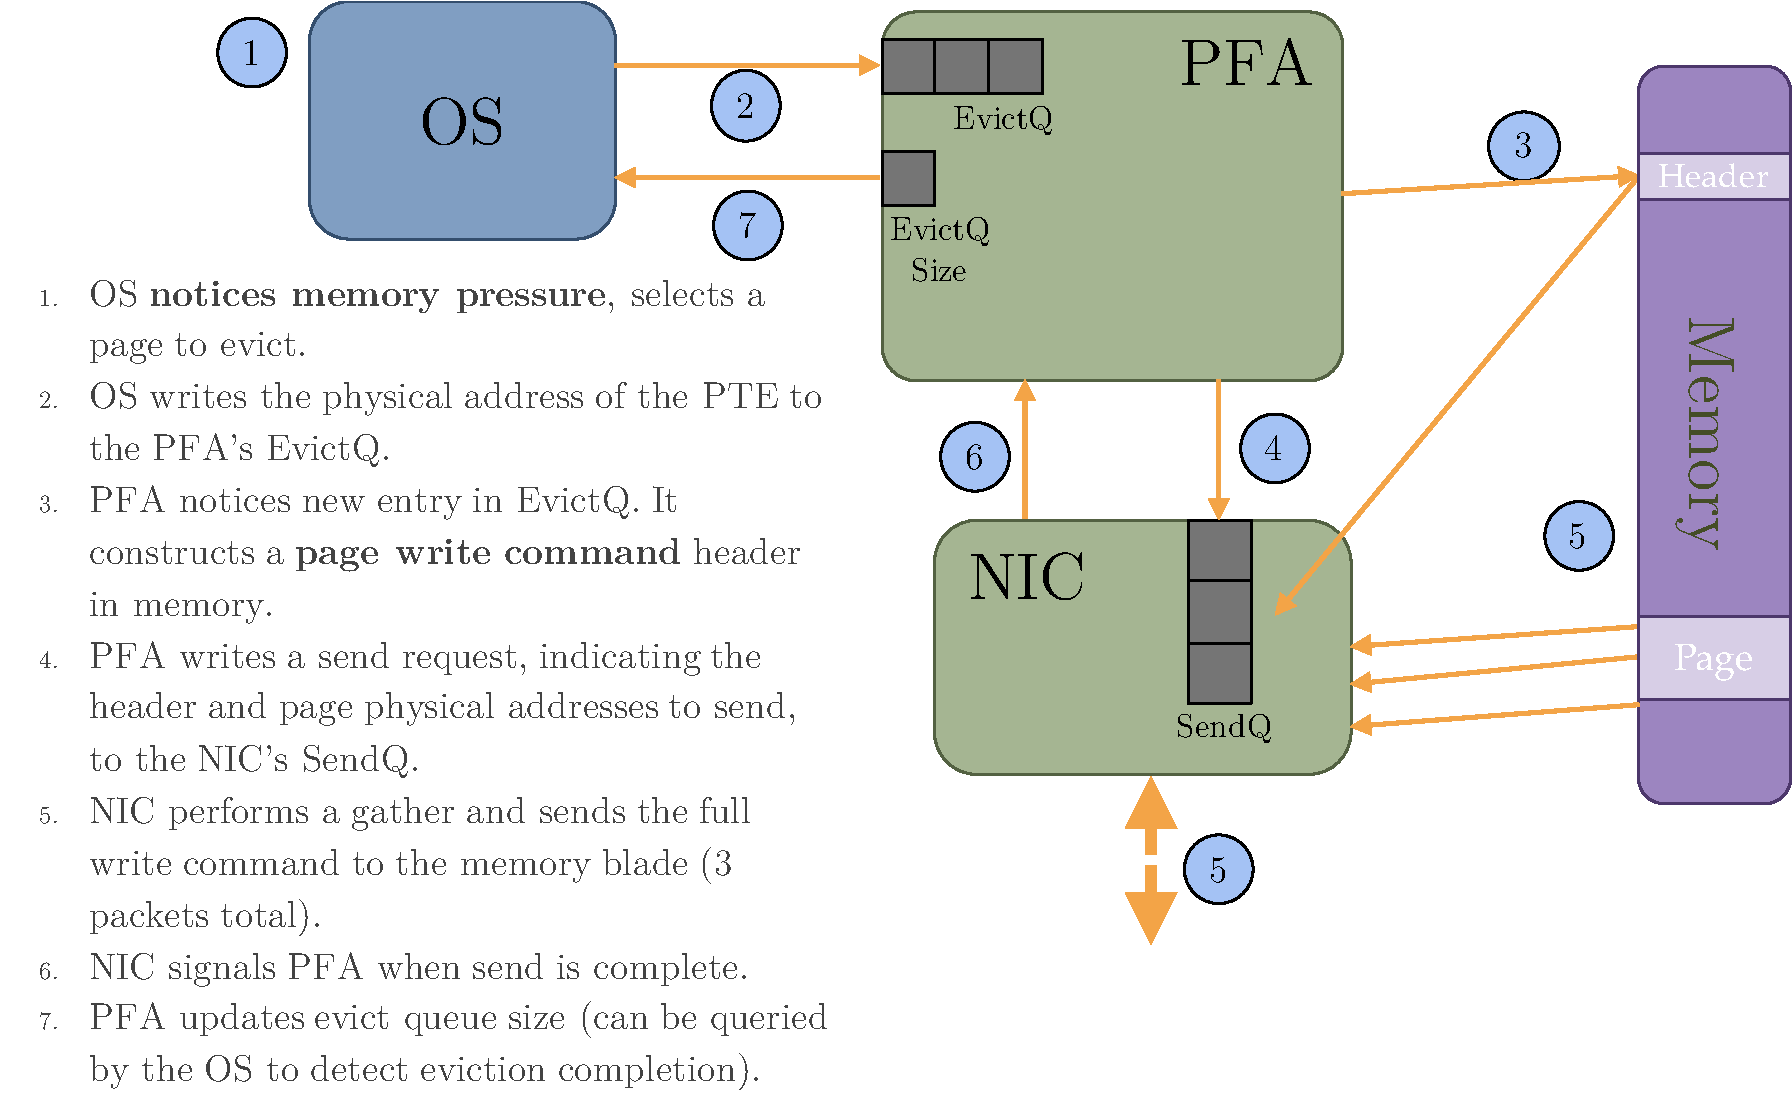
\includegraphics[width=\columnwidth]{figs/pfa_evict_detail.pdf}
  \vspace{-5mm}
  \caption{Detailed eviction flow}
  \label{fig:evict_detail}
\end{figure}

In addition to the three main queues, there are a number of other maintenance
registers that are used for querying queue status and initializing the PFA. See
appendix \ref{apx:pfa_spec} for a complete specification. I will mention one status
register here; the EVICT\_STAT register. When a page is placed on the evict
queue, the PFA begins transferring it to remote memory, but does not block
the OS. This allows the OS to perform useful work while the eviction is taking
place, potentially hiding some of the write latency. In order to re-use the
page frame, however, the OS must poll the EVICT\_STAT register to ensure the
write has completed.

\FloatBarrier

\paragraph{Fetch}
The primary function of the PFA is to automatically fetch pages from remote
memory when an application tries to access it. It does this by detecting page
table entries that are marked remote and transparently re-mapping them to the
next available free frame. The basic operation is as follows: 

\begin{outline}[enumerate]
    \1 Application code issues a load/store for the (now remote) page.
    \1 The PFA automatically and synchronously brings the page from remote
       memory and stores it in a free frame.
    \1 The PFA clears the remote bit in the \gls{pte}.
    \1 The PFA pushes the virtual address of the fetched page to the NewQ.
    \1 The application is restarted.
\end{outline}

Figure \ref{fig:fetch_detail} describes the process in more detail.
\begin{figure}[h] \centering
  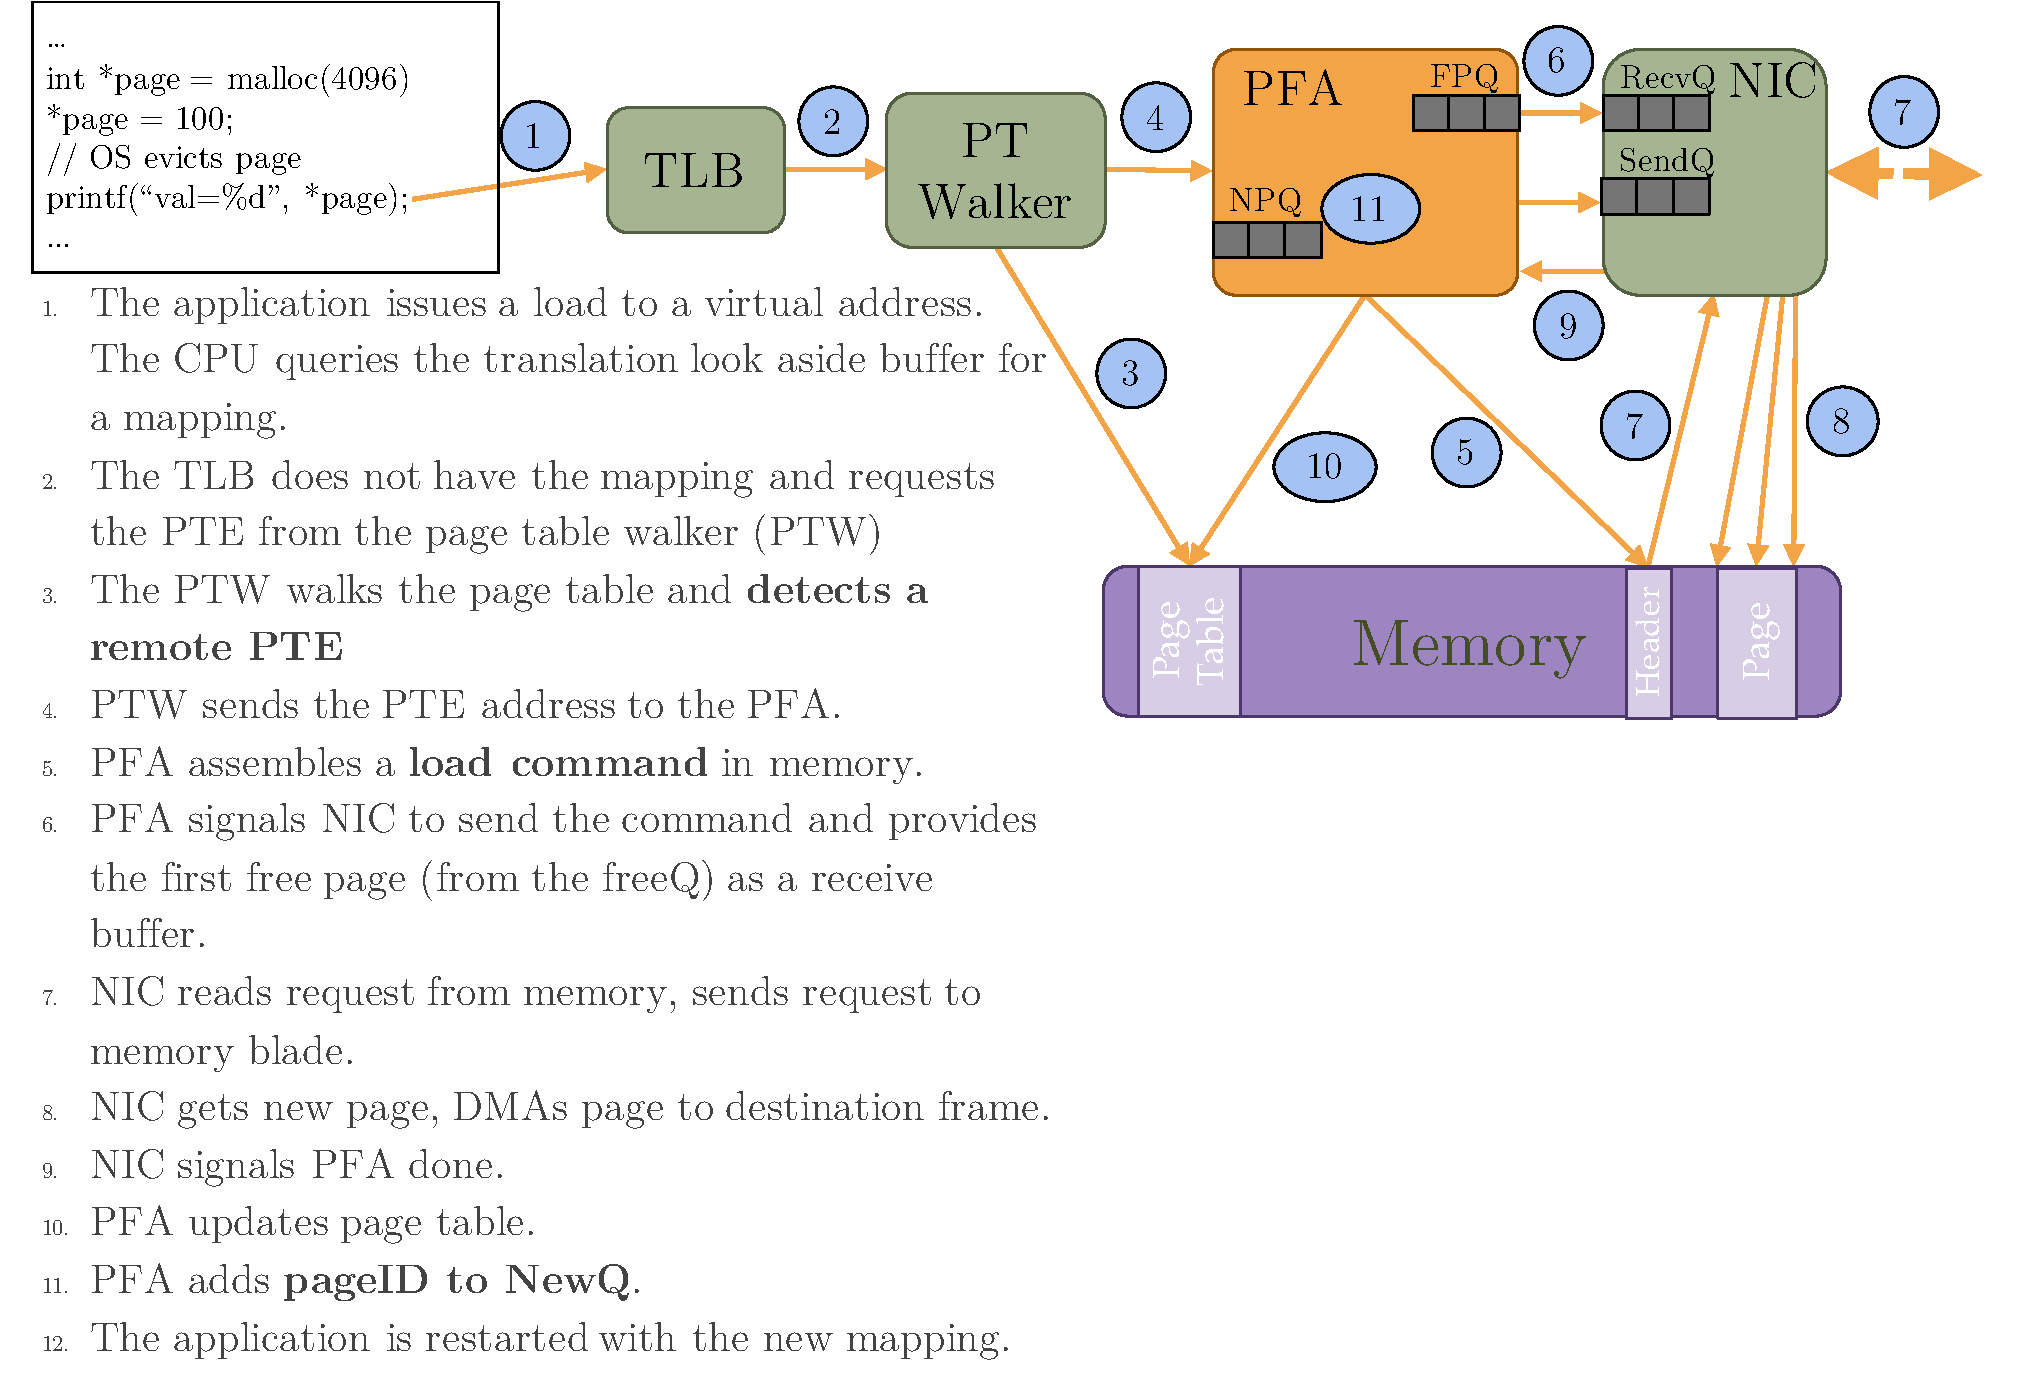
\includegraphics[width=\columnwidth]{figs/pfa_fetch_detail.pdf}
  \vspace{-5mm}
  \caption{Detailed fetch flow}
  \label{fig:fetch_detail}
\end{figure}
\FloatBarrier

\paragraph{Metadata Management}
The OS should ensure that there are sufficient free frames in the \gls{freeq} to
ensure smooth operation. If a remote page is requested and there are no free
frames, the PFA will trap to the OS with a conventional page-fault. The OS must
enqueue one or more free-frames before returning from the interrupt. This may
involve evicting pages synchronously in the page-fault handler.

Similarly, the OS needs to drain the new page queue periodically to ensure it
does not overflow. This will also trap to the OS with a conventional page
fault.

\subsubsection{Page Table Entry} \label{sec:remPTE}
The PFA uses a special PTE format for remote pages (Figure
\ref{fig:pte_format}). The fields are as follows:

\begin{outline}
  \1 \textbf{\gls{pgid}}: This acts as an address in remote memory for the remote
  page. It is used by the PFA to look up pages in remote memory, and for the OS
  to identify each page during bookkeeping.
  \1 \textbf{Prot}: This sets the protection bits that the PFA will use when
  fetching a page. These bits include things like read/write permissions, as
  well as other page metadata (see the RISC-V privileged architecture manual
  for more details \cite{riscv_priv110}).
  \1 \textbf{R}: This bit indicates that a page is remote (when the valid bit
  is clear).
  \1 \textbf{V}: This indicates whether a page is valid.  A valid page is
  currently in main memory and would not trigger a page-fault.  This is also
  referred to as the ``present bit'' in Linux.
\end{outline}

\begin{figure}[h]
  \centering
  \begin{bytefield}[endianness=big,bitwidth=0.016\linewidth]{64}
    \bitheader{0, 1, 2, 12, 40, 63} \\
    \bitbox{24}{Unused} & \bitbox{28}{Page ID} & \bitbox{10}{Prot} &
    \bitbox{1}{\tiny R} & \bitbox{1}{\tiny V} \\
  \end{bytefield}
	\caption{Remote PTE Format. The \textbf{Page ID} is a unique identifier of this page
  and serves as a remote memory address. The \textbf{Prot} field contains the permission
and metadata bits that should be set after a page is fetched (see the RISC-V
specification for details\cite{riscv_priv110}). The \textbf{R} bit indicates
that this page is remote while the \textbf{V} bit indicates that the PTE is not
a valid mapping (needed for backward compatibility).}
	\label{fig:pte_format}
\end{figure}

It is worth noting that the RISC-V instruction set manual specifies that all
bits other than the valid bit are considered ``don't care'' when the valid bit
is clear. This deviation from the standard may be problematic for some OSs, but
is compatible with the Linux kernel. Another interesting feature of this design
is the use of pre-defined protection bits. This includes a valid bit which can
be cleared by the OS before evicting to trigger a page fault on this page
immediately after fetching (a useful debugging feature). Also, bits 8 and 9 
are reserved for software by the RISC-V ISA and can aid the OS in bookkeeping
and debugging (see Section \ref{sec:linuxImpl}).

\subsubsection{Remote Memory Protocol}
When the PFA receives a request for a remote page from the PTW, it must
communicate with a remote \gls{memory blade} to retrieve the appropriate data.
It does this through a custom network protocol. This involves forming network
packets and interfacing with the NIC. For this project we assume an
Ethernet-based network with a \gls{mtu} of \SI{1500}{\byte} and a page size of
\SI{4}{\kilo\byte}, this is not fundamental to the design.  Figures
\ref{fig:write_protocol} and \ref{fig:read_protocol} show the basic operation
of the protocol. See appendix \ref{apx:memblade_spec} for a detailed
description of these packet types. Note that due to the \gls{mtu}, each page
takes 3 packets to transfer.
\begin{figure}[h]
    \centering
    \begin{sequencediagram}
        \newinst{c}{PFA}
        \newinst[6]{s}{Memory Blade}
        \mess[1]{c}{{fragment 1 (1468)}}{s}
        \mess[1]{c}{{fragment 2 (1468)}}{s}
        \mess[1]{c}{{fragment 3 (1460)}}{s}
        \mess[1]{s}{Ack}{c}
    \end{sequencediagram}
    \caption{Page Write. Note that each fragment contains a header containing a
    ``write'' opcode and destination \gls{pgid}, along with a unique
    transaction ID.}
		\label{fig:write_protocol}
\end{figure} 
 
\begin{figure}[h]
    \centering
    \begin{sequencediagram}
        \newinst{c}{PFA}
        \newinst[6]{s}{Memory Blade}
        \mess[1]{c}{{Read Request (PageID)}}{s}
        \mess[1]{s}{{fragment 1 (1468)}}{c}
        \mess[1]{s}{{fragment 2 (1468)}}{c}
        \mess[1]{s}{{fragment 3 (1460)}}{c}
    \end{sequencediagram}
		\caption{Page Read. Note that responses contain a header indicating the
    transaction ID of the corresponding read request.}
		\label{fig:read_protocol}
\end{figure} 

This protocol represents an initial design point that is suitable for a single
client/memory blade pair. We handle potentially out-of-order packets by
attaching sequence numbers and transaction IDs to each packet, but assume a
reliable network. While multiple clients could be supported with this protocol,
some interesting design challenges begin to appear. One issue is that of
fairness and congestion. A robust protocol would need some prioritization of
clients (perhaps assigned from a global allocator) and a back pressure mechanism
to ensure optimal behavior. It may be desirable, due to high access latencies,
to include some amount of compute in memory, whether that be traditional atomic
memory operations, or more general remote procedure calls. Another important component is that of
confidentiality and authentication. While it would be straight-forward to
encrypt payloads, this may interfere with atomics or other compute-in-memory
features. Headers present additional challenges. Simple encryption of headers
would not be sufficient because attackers could simply replay old requests to
modify application state. Some form of nonce (a unique number added to each
header) may be required. While the design of a memory blade represents an
interesting avenue of research, the design presented here is sufficient to
evaluate the PFA and I will leave further discussion to future work.



        
\section{Implementation} \label{sec_impl}
    \subsection{Hardware} \label{sec_hwImpl}
        \todo[inline]{Write Hardware Implementation section}
This section covers more concrete implementations of the PFA itself. I will cover both the software ISA simulator (work I did) and the RTL implementation (work Emmanuel did). It also includes a general introduction to the RISC-V ecosystem (including the SoC generator "RocketChip" and the simple in-order CPU "RocketCore").

\subsubsection{RISC-V and RocketChip}

\subsubsection{PFA Implementations}

    \subsection{Linux Integration} \label{sec_linuxImpl}
        We modified the Linux kernel (version 4.15\cite{linux}) to support the PFA. The
majority of software development was done using the functional simulator. Linux
is a mature open-source project with a long development history, resulting in
many Linux-specific terms. I will define these terms throughout this discussion
but you may refer to the glossary for a reference of terms.

\subsubsection{Non-PFA Paging in Linux} \label{sec:vanillaLinux}
I will now briefly describe how paging works in vanilla Linux. Note that the
kernel internally uses the term \gls{swap} in reference to all paging activity,
I will use these terms interchangeably. For a more complete discussion of
memory management in Linux, see \cite{linuxBook}. Figures
\ref{fig:vanilla_evict} and \ref{fig:vanilla_fetch} map out the steps involved
in evicting and fetching pages, respectively.

\paragraph{Page Reclaiming}
Linux manages memory limits on a per-task basis. In this case, a \gls{task}
refers to the kernel-specific abstraction of a process. Each task has its own
resource limits which are exposed to system administrators through the
\gls{cgroup} interface. When a task approaches its assigned limit of a certain
resource, it is throttled in a resource-specific manner. In the case of memory,
the kernel attempts to free task-assigned memory. It will first attempt to
shrink any file caches (especially clean disk blocks that can simply be deleted
without requiring any disk activity). If shrinking caches is not enough, the
kernel begins to page non-file backed pages (called ``\glspl{anonpg}''). This
is done using a pseudo-\gls{lru} eviction algorithm (Step 2 in Figure
\ref{fig:vanilla_evict}). Page reclaiming can be triggered
in one of two ways (Step 1). If a hard memory limit is met, but more memory is needed to
proceed, then page-reclaiming happens synchronously (called direct reclaim).
However, Linux tries to avoid this scenario by running a background thread
called \gls{kswapd} that begins reclaiming pages when the application reaches a
soft resource limit. \Gls{kswapd} is usually idle, but can be woken up when the
kernel detects a soft limit has been met. It also runs with a low priority to
avoid wasting resources on speculative evictions (the application may never hit
its hard limit).

\begin{figure}[h] \centering
  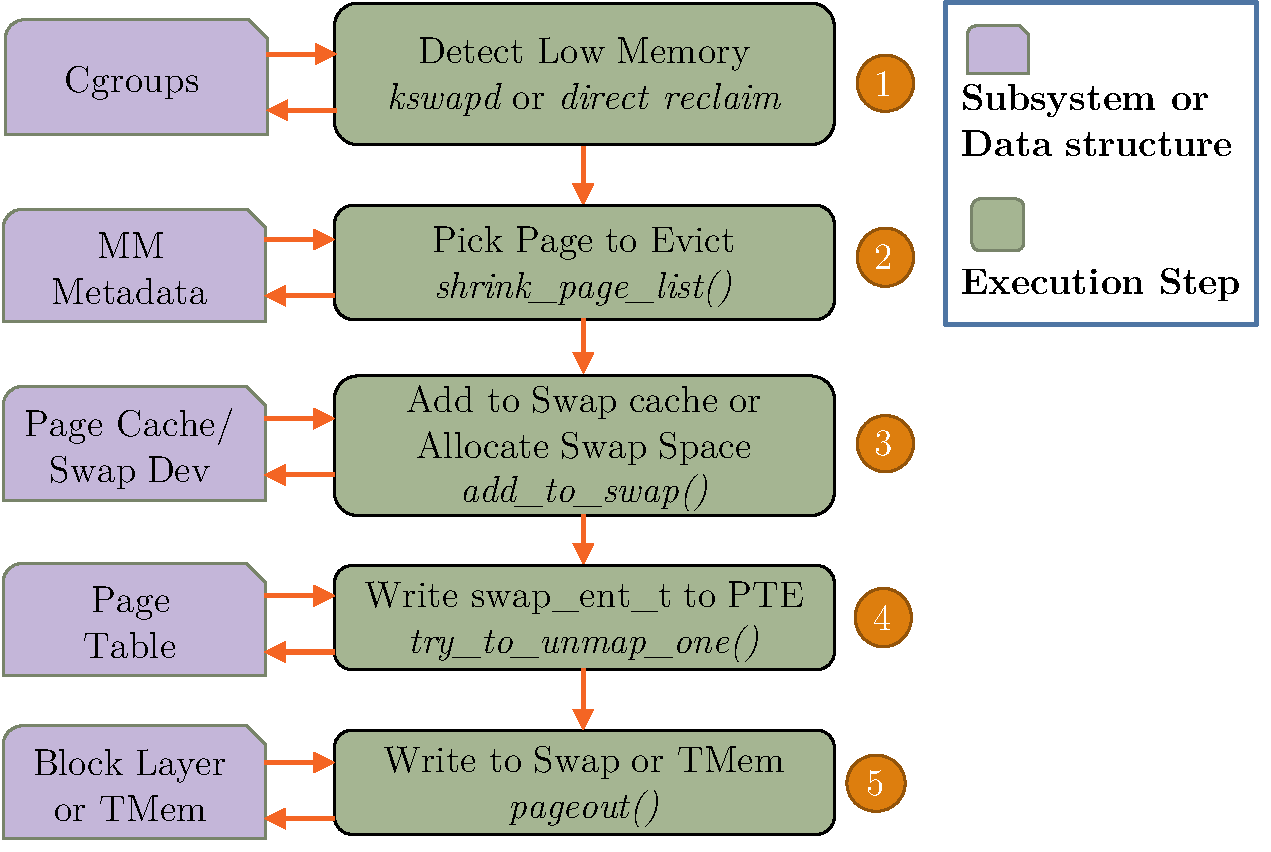
\includegraphics[width=0.7\textwidth]{vanilla_evict.pdf}
  \caption{Baseline Linux page eviction (reclaim) code path.}
  \label{fig:vanilla_evict}
\end{figure}

\paragraph{Page Eviction}
Paging was originally intended to use hard disks as backing store, and this is
reflected in the design of paging in Linux. To swap, one or more block
devices must be formatted and mounted as swap devices. Linux then uses the
block offset on this disk as a unique identifier for an evicted page (Step 3). In
order to support more complex paging schemes (such as page compression, or
heterogeneous memory), Linux introduced the \gls{tmem} layer\cite{tmem}. This
scheme still uses disk offsets as identifiers, but completely bypasses the block
layer. This is important because many optimizations in the block layer (e.g.,
write coalescing and block reordering) are not suitable for these alternative
paging devices. Evictions do not immediately result in writes to \gls{tmem} or
a swap device. Instead, pages are stored in a data structure called the swap
cache (Step 3). This swap cache helps reference count shared pages, and hedges
against poor eviction choices. Once a page is no longer physically available,
Linux replaces the corresponding \gls{pte} with a \gls{swpent} which clears the
valid bit, and uses the remaining bits to store the swap device ID (called
``type'' in the kernel) and block ID (called ``offset'') (Step 4).  When
changing a \glspl{pte}, most architectures require the OS to flush the
\gls{tlb}. This forces a page-table walk on the next access to this virtual
address. Finally, the kernel begins a write to the swap device in the
background (Step 5).

\paragraph{Page Fetch}

\begin{figure}[h] \centering
  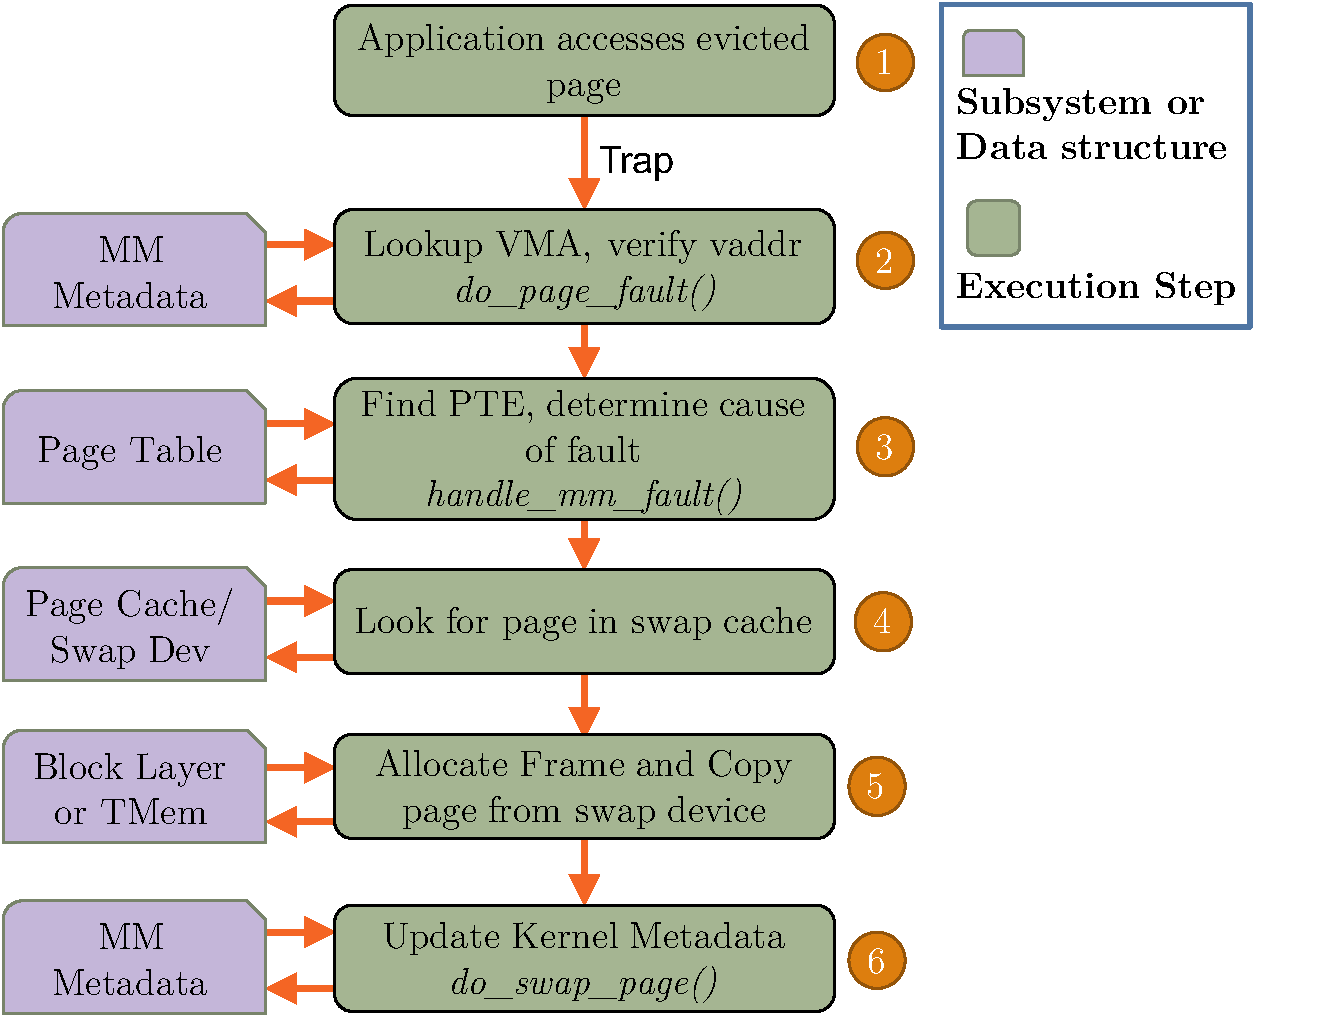
\includegraphics[width=0.7\textwidth]{vanilla_fetch.pdf}
  \caption{Baseline Linux page fetch code path.}
  \label{fig:vanilla_fetch}
\end{figure}

When a user program attempts to access a page that has been swapped out, the
\gls{ptw} notices the invalid PTE and issues a page fault trap to the OS (Step
1 in Figure \ref{fig:vanilla_fetch}). Note that the hardware does not examine
the remaining bits (the \gls{swpent} is purely a software construct). Upon
receiving a page fault, Linux first determines if the requested virtual address
has been assigned to this task. It does this by iterating through regions of
virtual memory called \glspl{vma} (Step 2). If a valid \gls{vma} is found, then
the OS begins a \gls{pgtbl} walk to locate the corresponding \gls{pte}. There
are several reasons that a page fault may occur, the OS must check the
\gls{pte} to determine the cause (Step 3). Assuming the cause was an invalid
\gls{pte}, the OS then searches the swap cache for this page (Step 4). This is
in case some other process that shares it has already brought it in. If the
page is not found, then a new frame is allocated and a transfer is initiated to
read the page from the swap device (Step 5). If the page is found in
\gls{tmem}, then the transfer occurs synchronously, otherwise the process
initiates the transfer and then yields to the scheduler, resulting in a context
switch. When the transfer is complete, the kernel changes the PTE from a
\gls{swpent} to a valid PTE with permissions defined by the \gls{vma}. Finally,
the kernel updates page-tracking meta-data (Step 6). This includes the \gls{lru} lists
maintained by the eviction algorithm, \gls{vma} membership, and a number of
other kernel subsystems. Note that several of these updates require
synchronization with other kernel threads. Once all bookkeeping is complete,
and the PTE is updated, the kernel flushes the \gls{tlb}, and restarts the
application.

\FloatBarrier 
\subsubsection{PFA Modifications}
The introduction of a PFA changes a number of the assumptions underlying
baseline paging behavior. Figure \ref{fig:linux_changes} summarizes these
changes.

\begin{figure}[h] \centering
  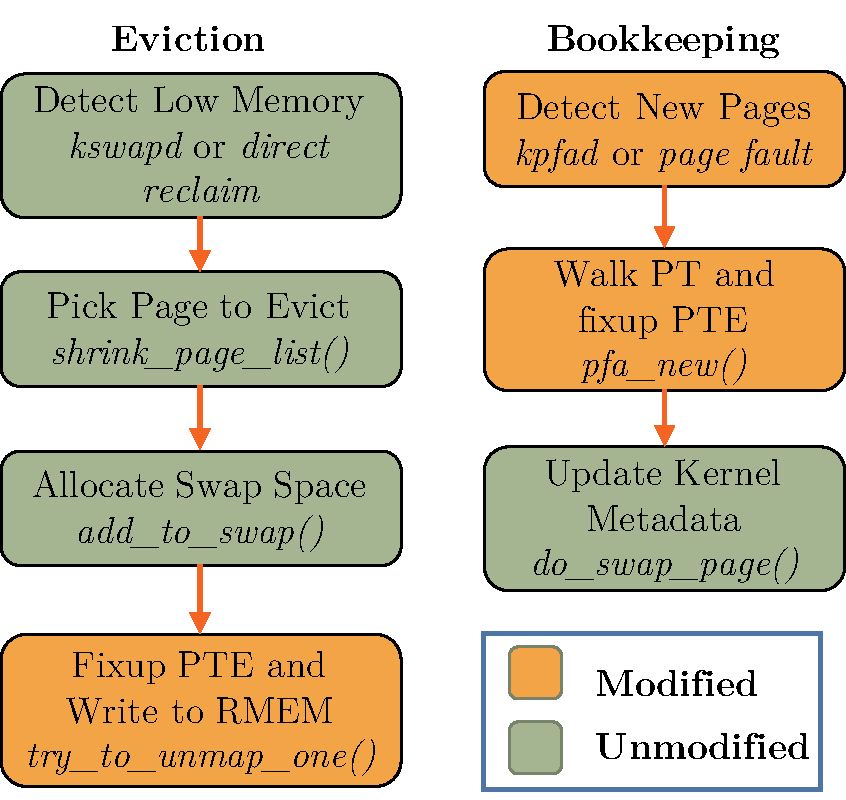
\includegraphics[width=0.5\textwidth]{linux_changes.pdf}
  \caption{Major changes to Linux paging to accommodate the PFA. Most
  subsystems could be re-used without change. On the eviction path, all that
  was changed was the PTE update (to write a remote \gls{pte} instead of a
  \gls{swpent}), and the write to disk (to write to remote memory instead). The
  bookkeeping path is now triggered either from the page-fault handler (due to
  a PFA service request) or from \gls{kpfad}. The core bookkeeping function
remains unmodified.}
  \label{fig:linux_changes}
\end{figure}

\paragraph{Frame Allocation and Permissions}
Linux uses the faulting virtual address to make a number of decisions during
the page fetch process. For instance, the permission bits are taken from the
\gls{vma}. \gls{vma} information is also used to decide which physical frame to
use (this is particularly important in NUMA systems). With the PFA, however,
the OS must decide on this information at \emph{eviction} time. Pre-allocating
physical frames is not an issue in our system because there is only one core,
and frame selection does not depend on the \gls{vma}. Permission bit selection
is more problematic. Our current approach is to assign permission bits to a
remote page based on the \gls{vma} permissions at the time of eviction, we then
update those permissions while performing bookkeeping. In practice, this is
unlikely to cause problems as permissions rarely change. Furthermore, Linux is
able to correct inappropriately restrictive permissions during page-faults.
However, there may be security concerns if permissions are made more
restrictive while a page is remote. This vulnerability exists in the window
between page fetch and bookkeeping. To mitigate this concern, the OS would need
to be modified to update remote PTEs when changing \gls{vma} permissions.

Under these simplifying assumptions, we are able to allocate frames
proactively. The current implementation always refills the \gls{freeq} during
bookkeeping. To simplify the bookkeeping procedure, we track
each allocated frame in a FIFO. This allows the bookkeeping code to simply pop
this FIFO to find which frame was used for each new page (the PFA always drains
the \gls{freeq} in FIFO order). Furthermore, this FIFO allows for aggressive
sanity checks that aided greatly in system debugging.

\paragraph{Asynchronous Bookkeeping}
In normal paging, the \emph{do\_swap\_page()} function is able to update meta-data as
soon as a page is fetched. With the PFA, we delay this bookkeeping for a
bounded but potentially non-trivial period of time. Many of these bookkeeping
tasks are in support of heuristics or resource accounting (e.g., LRU lists for
eviction, or memory utilization metrics). Delaying these tasks reduces the
accuracy of various algorithms, but does not result in incorrect behavior.
Others are needed for correct execution (e.g., \gls{vma} membership or shared
page tracking for copy-on-write). We address these correctness issues by
performing bookkeeping preemptively before accessing any of the related
algorithms. These tasks may be fairly common, but they are unlikely to actually
involve a recently fetched page. To avoid preemptively performing bookkeeping,
we use one of the reserved bits in the PTE protection field to indicate a page
that has been recently fetched but not yet processed. This bit gets set at
eviction time, but is cleared during bookkeeping.

\paragraph{Swap Device and Block ID Allocation}
Linux assumes that all swap activity is backed by a block device and it uses
the physical address on this device to identify all evicted pages. This block
ID is needed during the bookkeeping process to identify the page. To address
this problem we make a number of simplifying assumptions.

\begin{outline}[enumerate]
	\1 \textbf{A real swap device is available} (even though it is not used). We
		use a ram-based file system (ramfs) to trick the kernel into thinking it has
		a large disk attached. This uses no actual physical memory.
	\1 \textbf{There is only one swap device.} This allows us to not track device
		ID. This is achieved by making the ramfs sufficiently large to address all
		swap activity.
	\1 \textbf{Block IDs are contiguous on the integers $\mathbf{(0, 2^{28}]}$.}
		This allows us to pack the block ID into the remote PTE format (see Section
		\ref{sec:remPTE}). We achieve this by ensuring that the ramfs is the same
		size as our memory blade (and less than $2^{28}$ pages). Since block IDs
		correspond to physical offsets on the swap device, we are guaranteed to
		never see an invalid block ID.
\end{outline}

While these assumptions hold, we are able to compress the \gls{swpent} into a
\SI{28}{\bit} PageID by eliding the type, and using the offset directly.
Finally, we avoid overheads in the block layer by implementing the PFA as a
\gls{tmem} device. Since bookkeeping is asynchronous, and eviction occurs
earlier in the process (due to ordering constraints with PTE modifications),
this \gls{tmem} plugin simply returns immediately. The current implementation
evicts synchronously. This is because the expected write time is much smaller
than a scheduling quantum and asynchronous eviction would result in wasteful
context switches. Future implementations may attempt to overlap eviction with
low-latency tasks such as bookkeeping.

\subsubsection{kpfad} \label{sec:kpfad}
The most basic implementation of PFA support in Linux simply performs
bookkeeping tasks whenever the internal queues of the PFA fill up. This
effectively batches page bookkeeping, but it does not allow the kernel to
choose when the bookkeeping occurs. To leverage idle periods in
program execution, or unused hardware threads, we implement a background
bookkeeping daemon called \gls{kpfad}. \Gls{kpfad} is triggered by an adaptive
timer that attempts to discover the average time between full queues. It does
this by increasing the wait time by a small amount every time it runs, and
decreasing the time whenever the application is interrupted due to full queues. 
While \gls{kpfad} gives increased flexibility and efficiency on a lightly
loaded system, it causes strictly more overhead than interrupt-driven
bookkeeping when the application has enough work to keep all hardware threads
busy (since the adaptive timer is not perfect). To avoid this, \gls{kpfad} is run
with very low priority (similar to the page-out daemon \gls{kswapd}). Unlike
\gls{kswapd}, however, \gls{kpfad} does not get triggered by a soft limit. We expect
the adaptive timer scheme, coupled with low priority, to be sufficient to avoid
significant overhead.

\subsubsection{Baseline Swapping}
We modified Linux to use the remote memory blade while paging. This was done by
implementing a software interface to the remote memory blade as a \gls{tmem}
device. The swapping mechanism uses a custom NIC driver that provides zero-copy
semantics and bypasses the normal Linux networking stack. 



\section{Evaluation} \label{sec_eval}
    \subsection{Experimental Design} \label{sec_expDesign}
        \todo[inline]{Experimental Design}
This section will cover FireSim, network parameters, and the memory blade model we're using. It will also cover the benchmarks. Benchmarks will include at least a subset of Spec and a genome assembly benchmark, but hopefully also some neural networks and possibly even a distributed reinforcement-learning application (Ray).
    \subsection{End-to-End Performance} \label{sec_fullPerf}
        \todo[inline]{Write End-to-End Performance section}
This is the key experiment. I will run the benchmarks with and without the PFA, while also varying network properties. Given prior experiments and my understanding of our implementation, I expect to see modest improvements here. The base-case will be swapping to a RAM disk (full linux SW stack) with delays added to simulate network latency.

I would really like to have a comparison with a fully hardware-managed DRAM cache. I'm not sure how realistic that really is. We might be able to plug some sort of cache simulator into Rocket, or we could use published numbers for DRAM cache performance. I'm not sure what the best course of action is on this.
    \subsection{Software Overheads} \label{sec_swOverhead}
        \todo[inline]{Write Software Overheads section}
This section will explore where time is going when paging with the PFA. How much time is spent in bookkeeping? Does putting kpfad on another core help? How many page faults is the PFA not able to eliminate due to Linux design choices (e.g. shared pages will fault anyway, so will read-only pages)? Initial experiments suggest a significant number of page faults make it to the OS. We also have to prematurely do bookkeeping inline at times due to correctness constraints in the kernel.

This section also serves as a bit of ``future-work'' in that I will hopefully identify potential optimizations (or describe optimizations I have done due to measurement and experimentation).
    \subsection{Impact of CPU Micro-Architecture} \label{sec_uarchImpact}
        \todo[inline]{Write Micro-Architectural Impacts section}
This section explores how our choice of CPU and SoC impacted our results. Previous work has shown that page faults are relatively cheap on simple in-order cores like Rocket. We may do some experiments with BOOM (the out-of-order RISC-V core), but it's not clear we'll be able to do full PFA experiments with it before the end of the semester. We may use some models to explore how increased page fault costs, increased application complexity, or increased core counts might change our conclusions.
        
\section{Conclusion} \label{sec_conclusion}
    \todo[inline]{Write Conclusion}
Obviously this will depend on our final results. I may try to lay out the conditions under which this design point makes sense (a la ``Gang Scheduling Not Worth It...Yet''). This will also be an opportunity to step back and look at the larger disaggregated memory landscape. We really started this project as a way of feeling out the limits of performance and getting concrete numbers for evaluating if disaggregation makes sense at all. At the end of the day, cache-like approaches will be highly desirable in a disaggregated setting, we need to understand its limitations.

\listoftodos

\bibliographystyle{abbrv}
\bibliography{pfa}

\end{document}
